\documentclass[9pt,a4paper,twocolumn,uplatex]{jsarticle}
%\usepackage{layout}
\usepackage[top=20mm,bottom=20mm,left=15mm,right=15mm]{geometry}
\usepackage{amsmath,amssymb}
\usepackage{bm}
\usepackage[dvipdfmx]{graphicx}
\usepackage{ascmac}
\renewcommand{\baselinestretch}{0.65}
\setcounter{page}{21} %[重要]自分のページ番号に変更すること。
\title{\textbf{11.畳み込み辞書学習を用いたクラス分類の検討}}
\author{$[$\textbf{機械・電気システム工学専攻}$]$\textbf{平川智也}\\$[$\textbf{指導教員}$]$\textbf{黒木祥光 教授}}
\date{\today}

\makeatletter
\def\@maketitle{%
	%\newpage\null
	\vskip 2em%
	\begin{center}%
		\let\footnote\thanks
		{\Large \@title \par}%
		\vskip 1.5em%
	\end{center}% 追加
	\mbox{}\hfill%% 追加
	{\large
		\lineskip .5em%
		\begin{tabular}[t]{r}%
			\@author
		\end{tabular}\par}%
	\par\vskip 1.5em}
\makeatother

\begin{document}
\setlength{\abovedisplayskip}{2pt}
\setlength{\belowdisplayskip}{2pt}
\twocolumn[
\maketitle
	\textbf{Abstract}:In this study, we propose a novel classification method based on Convolutional Dictionary Learning (CDL) and Cone Restricted Subspace Method (CRSM). 
	Our method extracts shift-robust-feature by using power spectra of sparse coefficients  obtained from CDL.
	Then the spectra receive linear variations of nonnegative coefficient because of nonnegativity of the spectra and they make cone-shaped space generally.
	Our method introduces CRSM which uses the traits of the spectra.Experiments on handwritten image classification shows that information of frequencies improves classification accuracy, and that our method achieves higher classification accuracy undersmall-number-training dataset. 
\vspace{2.5mm}
]

\section{概要}
本研究では,畳み込み辞書学習および錐制約部分空間法を用いたクラス分類法を提案する.
提案法では畳み込み辞書学習で得られたスパース係数のパワースペクトルを用いることで,物体の位置ずれに頑健な特徴を抽出する.
得られた特徴は非負の制約を受けるため,多くの場合,加法とスケール変化,すなわち非負結合係数による線形変動を受ける.
これは一般に原点を頂点とする錐の形状をなす.
提案法では上記の特性を利用した錐制約部分空間法を適用する.
実験から手書き数字データの分類に適用し,係数の周波数情報を利用することの優位性及び,訓練データが少ないケースでの提案法の優位性が示された.

\section{はじめに}
畳み込み辞書学習(Convolutional Dictionary Learning:CDL)は従来のスパース係数と辞書の線形結合で入力信号を再現する辞書学習と比較し,画像をパッチ分割せずに特徴抽出できることや,周波数領域の計算によって計算の高速化ができること,畳み込みニューラルネットワーク(CNN)の畳み込み層との構造上の類似などから,画像処理分野で研究が進められている\cite{csc}.
CDLは入力信号を複数のフィルタとスパース係数に分解する.
フィルタは画像の局所的な特徴を表し,係数はフィルタの表す特徴が画像のどの位置に顕在するかを表す.
したがって入力信号がシフト変動を受けた場合には係数も入力信号と近しいシフト変動を受ける.
そこで本研究ではスパース係数のパワースペクトルを分類における特徴として用いることにより,シフト変動に頑健な分類器を構築する.
パワースペクトルは非負値をとるため,分類問題における各クラスにおける特徴は原点を頂点とする錐の形状をなすと仮定し,錐制約部分空間法(Cone  Restricted Subspace Method:CRSM)\cite{subspace}を適用する.
ここで,特徴ベクトル空間でサンプルベクトルが張る凸錐は次式で定義される.
\begin{equation}
C:=\{\bm x|\bm x=\sum_{i=1}^{N}\alpha_i\bm\xi_i=\Xi\bm\alpha\,~\bm\alpha\geq\bm 0\}
\end{equation}
$N$ はサンプルベクトル$\bm\xi_i\in\mathbb R^d$ の数,$\alpha_i$ は非負結合係数で,$\Xi=[\bm\xi_1,\bm\xi_2,...,\bm\xi_N],~\bm\alpha={}^t[\alpha_1,\alpha_2,...,\alpha_N]$ である.
錐は部分空間における結合係数に非負制約を付与したものであり,部分空間と同様にスケール変化やベクトルの加法に対して閉じた表現となっている.CRSMでは入力ベクトルと錐のなす角度により識別を行う.角度θは特徴ベクトルとその錐Cへの正射影ベクトルのなす角度と定義される.

\section{畳み込み型辞書学習}
CDL では以下の最適化問題を解くことによって入力信号$\bm y\in\mathbb R^D$をフィルタ$\bm d_i\in\mathbb R^d$とスパース係数$\bm x_i\in\mathbb R^D~(i=1,2,...,C)$に分解する.
\begin{eqnarray}
\label{equation:problem}
\bm d, \bm x=\arg\min_{\bm d, \bm x}\frac{1}{2}\|\bm y&-\sum_{i=1}^{C}\bm d_i*\bm x_i)\|_2^2+\lambda\sum_{i=1}^{C}\|\bm x_i\|_1\nonumber\\
&~~\text{s.t.}~~\bm d\in C_d,~\bm x\in C_x
\end{eqnarray}
ここで$C_d,~C_x$はそれぞれフィルタ,係数に対する制約集合である.
$*$は巡回畳み込みの操作を表し,$\|\cdot\|_1$ は$\ell_1$ノルムを表す.
問題(\ref{equation:problem})は以下の2つの凸最適化問題に分割される.

\begin{equation}
\label{equation:d_update}
\bm d=\arg\min_{\bm d}\frac{1}{2}\|\bm y-\sum_{i=1}^{C}\bm d_i*\bm x_i)\|_2^2~~\text{s.t.}~~\bm d\in C_d
\end{equation}
\begin{equation}
\label{equation:x_update}
\bm x=\arg\min_{\bm x}\frac{1}{2}\|\bm y-\sum_{i=1}^{C}\bm d_i*\bm x_i)\|_2^2+\lambda\sum_{i=1}^{C}\|\bm x_i\|_1~~\text{s.t.}~~\bm x\in C_x
\end{equation}
問題(\ref{equation:d_update}),(\ref{equation:x_update})を交互に解くことで解を得るが,これらの問題は凸最適化問題の反復解法であるADMM(Alternating  Direction  Method  of  Multipliers)\cite{admm}を用いて最適化される.
最適化の際,巡回畳み込みの操作についてフーリエ領域で計算を行うことにより,処理の高速化が可能である\cite{csc}.

\section{提案法}
提案法では問題(\ref{equation:problem})で得たスパース係数$\bm x_i$ のパワースペクトルを特徴ベクトルと見做す.
$\bm x_i$ は本来2次元の配列として表現されるため,2次元FFTを用いて周波数領域での表現$X\in\mathbb C^{h\times w}$を得る.
ここで$\bm x_i$ のパワースペクトル$P(\bm x_i)\in\mathbb R_+^{h\times w}$は以下のように定義される.
\begin{equation}
[P(\bm x_i)]_{i,j}=[\bar{X_{i,j}}\cdot X_{i,j}]_{i,j}
\end{equation}
ここで$X_{i,j}$は行列のi行j列の要素を表し,$\bar{}~,~\cdot$はそれぞれ複素共役,エルミート内積を表す.
パワースペクトルはその信号中に含まれる周波数成分の強度を示すもので,シフト変動に頑健である(図\ref{fig:spectra}).
\vspace{-1.5mm}
\begin{figure}[htb]
	\centering
	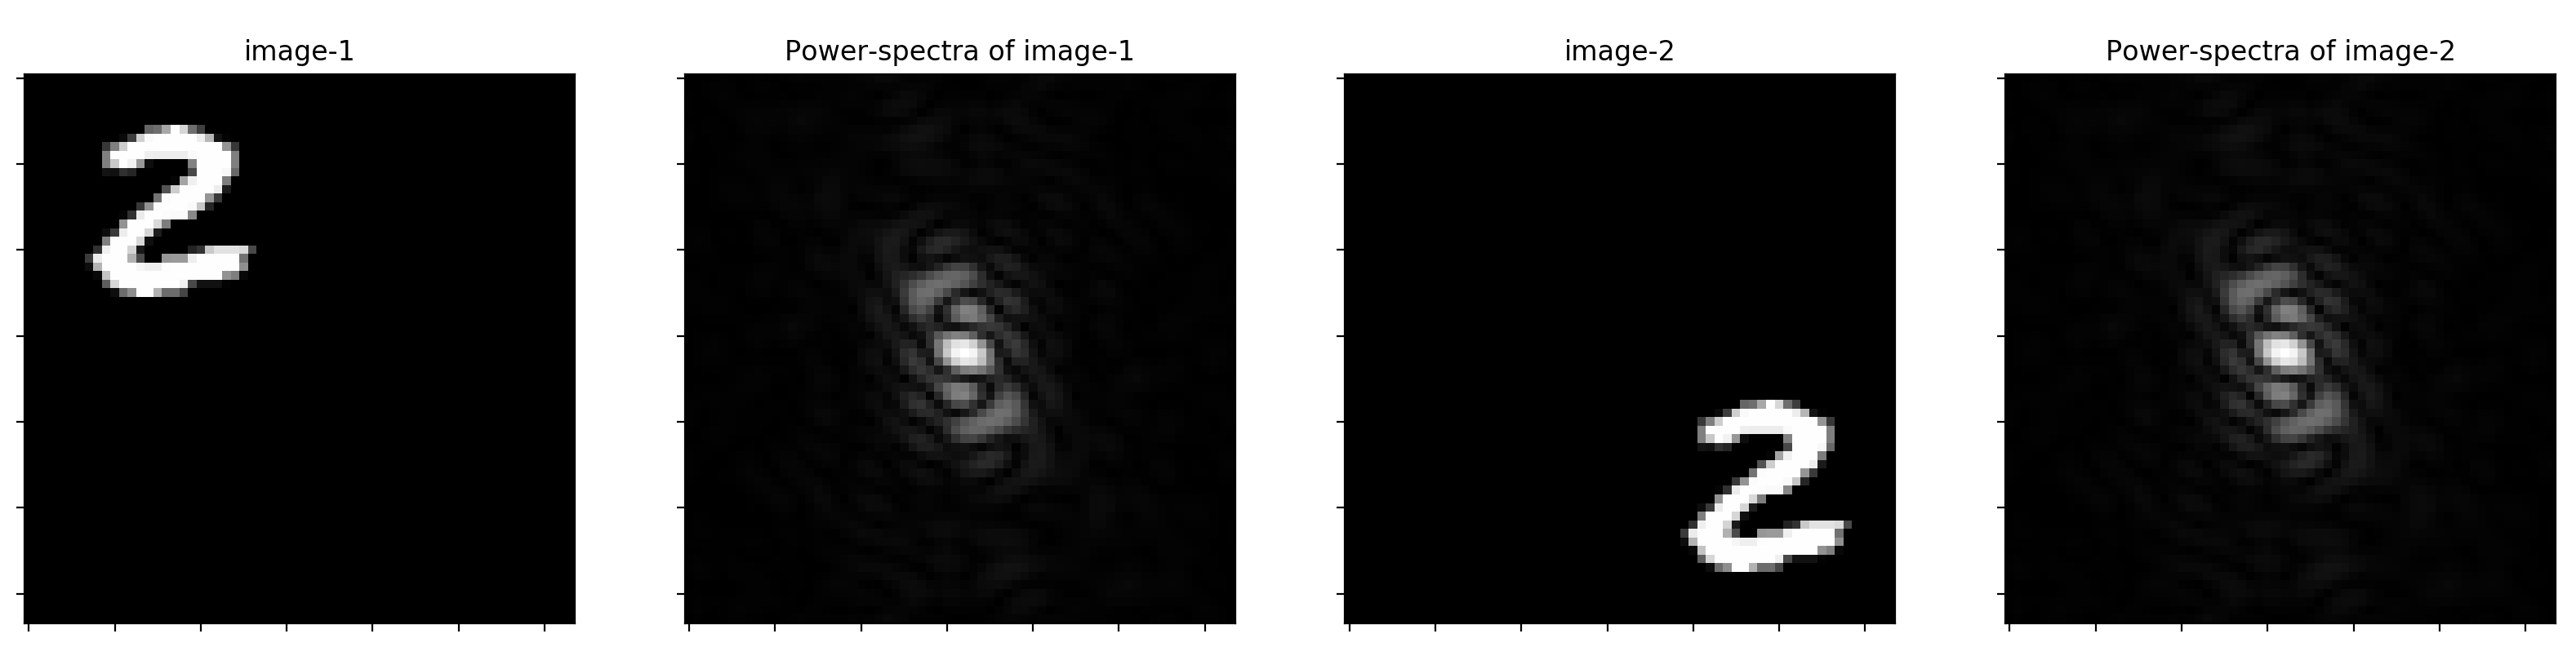
\includegraphics[width=\linewidth]{spectra.png}
	\caption{シフト変動させた画像に対するパワースペクトル}
	\label{fig:spectra}
\end{figure}
式(5)に示すパワースペクトルの各要素は非負値をとることから部分空間法ではなく錐制約を課した部分空間法を用いるのが好ましいと考えられる.
また部分空間法はCNNと比較して,クラス数の変動が起きた際にネットワークの再学習の必要がなく,新たなクラスの張る錐を構築するのみでよいため,クラス数の変動に頑健である.
錐の基底の構築方法として様々な方法が提案されている\cite{cones}が,本研究では非負値行列因子分解(Nonnegative Matrix Factorization:NMF)\cite{nmf}を用いる方法と,包括凸錐を用いる方法を採用する.
以下に具体的な方法を示す.

\subsection{NMFによる錐の構成方法}
NMF では,以下の最適化問題を解くことで,N個の非負特徴ベクトル$\bm y_i\in\mathbb R_+^d$ を列ベクトルとする非負値行列$Y=[\bm y_1, \bm y_2,...,\bm y_N]\in\mathbb R_+^{d\times N}$ を2つの非負値行列$H=[\bm h_1,\bm h_2,...\bm h_K]\in\mathbb R_+^{d\times K}$と$X=[\bm x_1,\bm x_2,...,\bm x_N]\in\mathbb R_+^{K\times N}$に分解する.

\begin{equation}
	H,X=\arg\min_{H,X}c(H,X)~~\text{s.t.}~~H_{i,j}\geq 0,~X_{i,j}\geq 0
\end{equation}

ここで$c(H,X)$はコスト関数を表し,本研究ではフロベニウスノルム$\|Y-HX\|_F^2$を用いた.
このとき$H$の各列ベクトルは錐の基底ベクトルをなし,$X$の各列ベクトル$\bm x_i$は各特徴ベクトル$\bm y_i$に対する結合係数であると解釈できる.


\subsection{包括凸錐の構成方法}
包括凸錐は非負特徴ベクトル群に対して主成分分析を行うことによって,それらを包括する凸錐を構築する.
先ず,特徴ベクトル群を単位超球面上に射影する.
それらの自己相関行列に対して固有値分解を施し,得られた固有ベクトルを固有値の大きさに従い降順で並べると,第1固有ベクトルは原点からの錐の方向を示し,それに直交する第2以降の固有ベクトルは超球面上の分布の広がり具合を示す.
よって第2以上の各固有軸上で分布を包括する2点を選ぶことで分布を包括する凸包を構成する(図\ref{fig:howtomakeccone}).
各固有軸に対して以下の2つの基底ベクトルが定まる.
\begin{equation}
\bm e_{i+}=\bm s_1+k\sqrt{\lambda_i}\bm s_i
\end{equation}
\vspace{-2.5mm}
\begin{equation}
\bm e_{i-}=\bm s_1-k\sqrt{\lambda_i}\bm s_i
\end{equation}
ここで$\bm s_i,~\lambda_i$はそれぞれ第$i$固有ベクトル,固有値を表し,第2以降の固有軸上での分布の分散は固有値$\lambda_i$で与えられる.
ここでは外れ値の値を考慮し,各軸上での標準偏差の$k$倍の点を端点として選んでいる.
主成分分析において採用する次元数$r$は第2以降の固有値の累積寄与率$\nu_i=\sum_{j=2}^{i}\lambda_i/\sum_{j=2}^{d}\lambda_j$によって定めることで,包括凸錐の基底ベクトルは$2(r-1)$個得られる.
\vspace{-1.5mm}
\begin{figure}[htb]
	\centering
	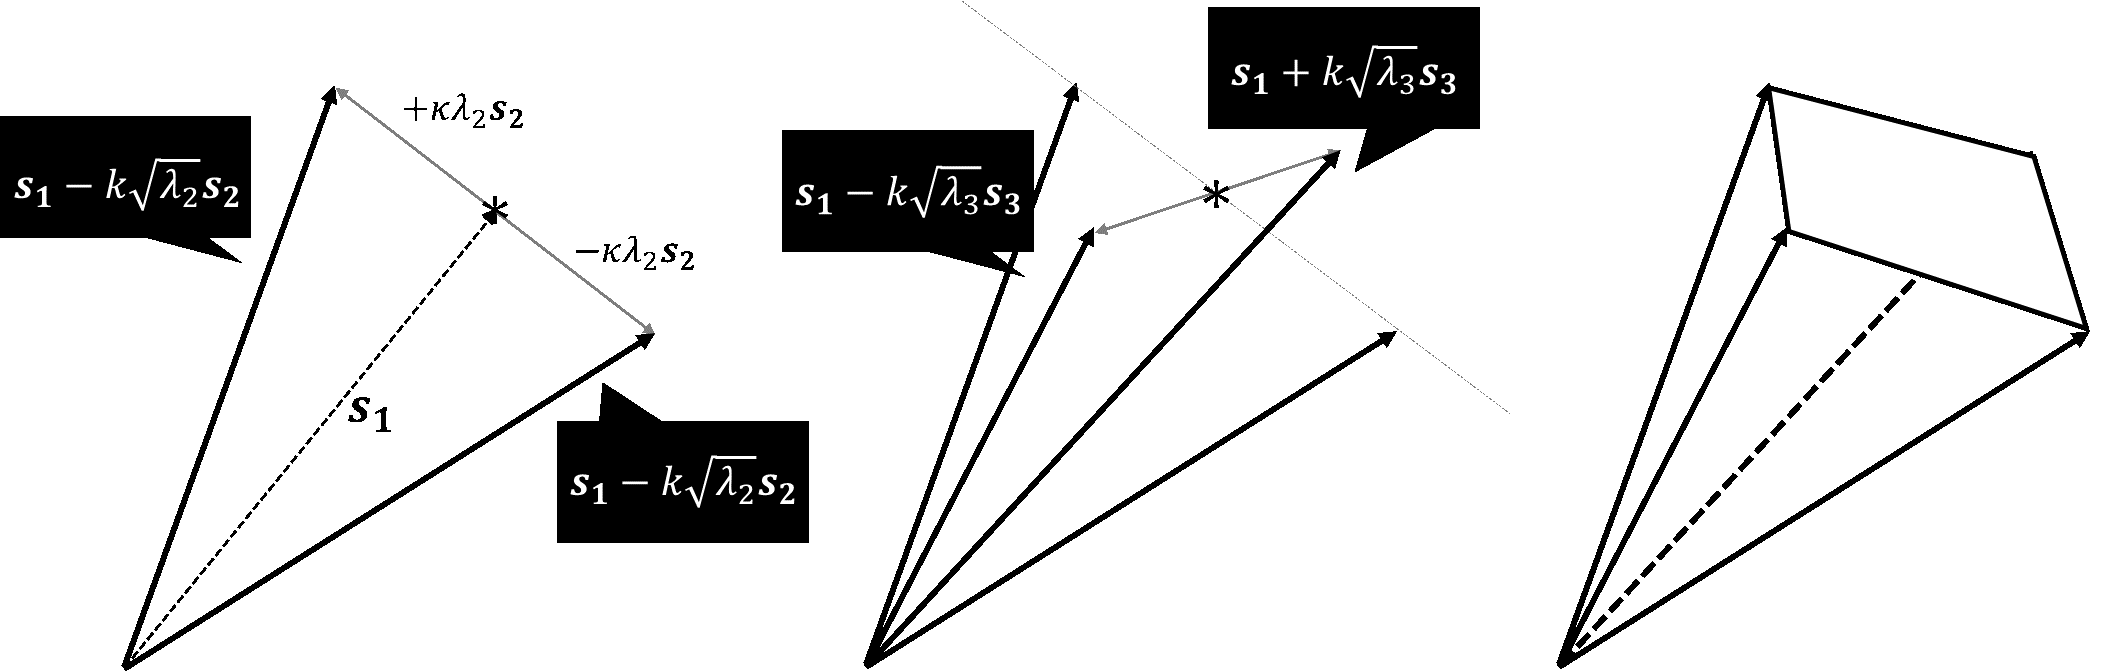
\includegraphics[width=\linewidth]{makeCone}
	\caption{包括凸錐の構成方法}
	\label{fig:howtomakeccone}
\end{figure}
\vspace{-1.5mm}
\section{実験}
提案法の有用性を示すために,手書き数字データセットであるMNISTの分類に適用した.
比較対象として,非負制約付きCDLによって得られた係数と,そのパワースペクトルをそれぞれベクトル化し,フロベニウスノルム規準のNMFによって256次元まで次元削減したものを特徴ベクトルとした.
分類器は錐制約部分空間法のほかに3層ニューラルネットワーク(NN),Support Vector Machine(SVM)を用いて分類精度を算出した.
訓練用画像は1000枚に固定し,訓練用画像は100, 200, 300, 400, 500, 1000枚と変動させた.
訓練用画像枚数が200枚および1000枚における実験結果を図\ref{fig:result-200},図\ref{fig:result-1000}に示す.
\begin{figure}[htb]
	\centering
	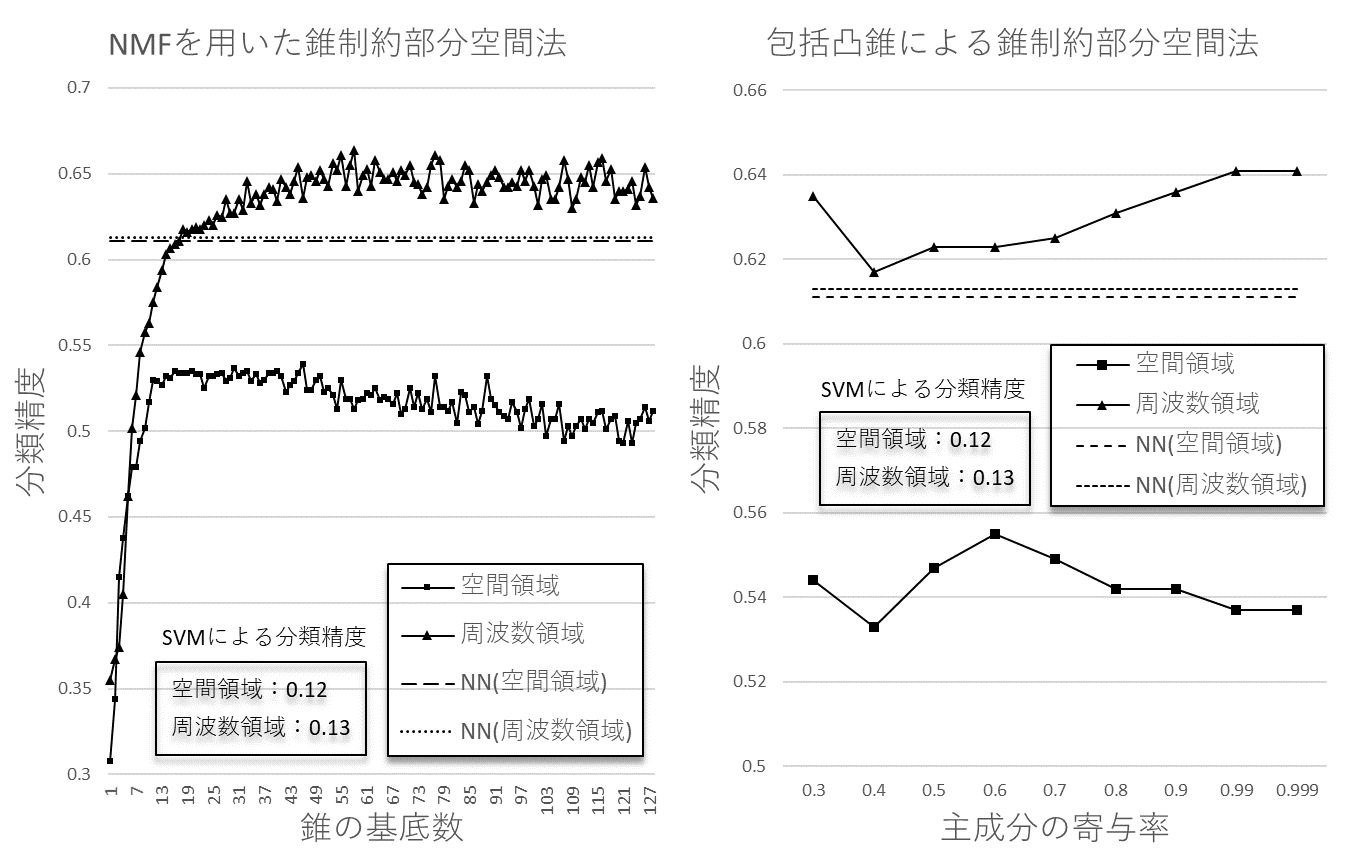
\includegraphics[width=\linewidth]{result-200}
	\caption{訓練画像200枚での実験結果}
	\label{fig:result-200}
\end{figure}
\begin{figure}[htb]
	\centering
	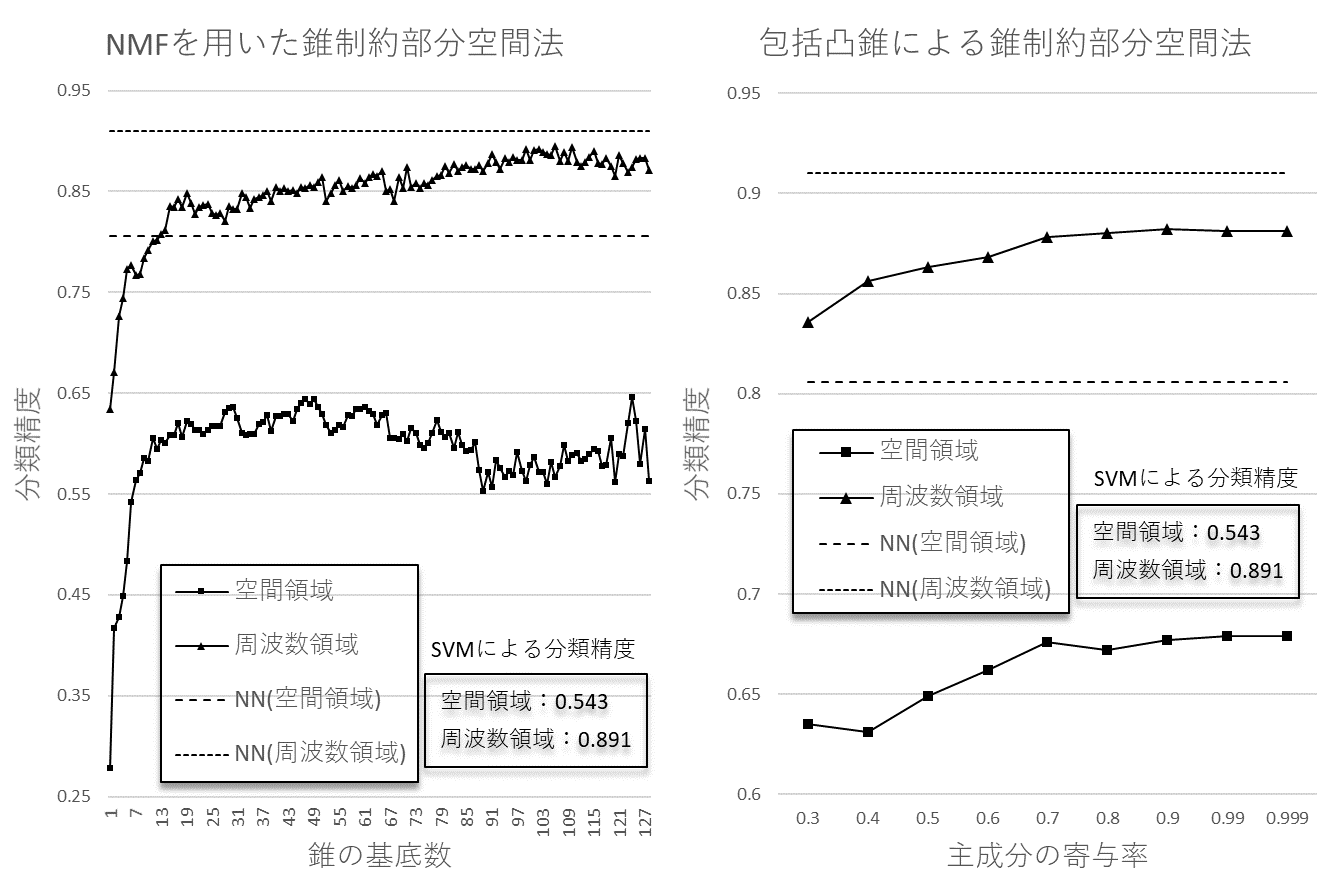
\includegraphics[width=\linewidth]{result-1000}
	\caption{訓練画像1000枚での実験結果}
	\label{fig:result-1000}
\end{figure}
結果より,スパース係数のパワースペクトルを用いる提案法がスパース係数をそのまま特徴とする手法よりも高い認識精度を示した.
これは画像の周波数成分を特徴として用いることでシフト変動に対する頑健性が増したためと考える.
また,訓練用画像枚数が少ない状況下において,3層NNよりも高い認識精度を示す.

\section{結言}
本研究では畳み込み辞書学習によって得られたスパース係数のパワースペクトルを特徴とし,錐制約部分空間法を用いた分類器を設計した.
実験結果より,パワースペクトルを特徴として用いることの有用性,また錐制約部分空間法が,データ数が少ない状況下における分類手法に適していることが示された.
今後の課題として,畳み込み辞書学習の多層化,得られた特徴の次元削減の方法,大規模データセットにおける挙動解析などがあげられる.
\begin{small}
\begin{thebibliography}{}
	\bibitem{csc} Bristow, Hilton, Anders Eriksson, and Simon Lucey. "Fast convolutional sparse coding." Proceedings of the IEEE Conference on Computer Vision and Pattern Recognition. 2013.
	\bibitem{admm} Boyd, Stephen, et al. "Distributed optimization and statistical learning via the alternating direction method of multipliers." Foundations and Trends® in Machine learning 3.1 (2011): 1-122.
	\bibitem{subspace} 福井和広,”部分空間法の今昔(下),”情報処理学会,vol.49(6),pp.680-685,Jun. 2008.
	\bibitem{cones} 小林匠,大津展之,”パターン識別のための錐制約部分空間法,”電子情報通信学会論文誌,vol.J92-D1,pp.104-111,Jan. 2009.
	\bibitem{nmf} 亀岡弘和,“非負値行列因子分解,”計測と制御,vol.51, no.9, pp.835-844, Sep. 2012.
\end{thebibliography}
\end{small}


\end{document}